\documentclass[conference]{IEEEtran}
\usepackage{times}

% numbers option provides compact numerical references in the text. 
\usepackage[numbers]{natbib}
\usepackage{multicol}
\usepackage[bookmarks=true]{hyperref}
\usepackage{amsmath}
\usepackage{amssymb}
\usepackage{graphicx}
\usepackage{subfigure}
\usepackage{algorithm}
\newtheorem{theorem}{Theorem}
\newtheorem{remark}{Remark}
\newtheorem{lemma}{Lemma}
\newtheorem{definition}{Definition}

\pdfinfo{
	/Author (Homer Simpson)
	/Title  (Robots: Our new overlords)
	/CreationDate (D:20101201120000)
	/Subject (Robots)
	/Keywords (Robots;Overlords)
}

\begin{document}

% paper title
\title{Optimal Measurement Scheduling for Cooperative Localization in Resource-constrained Conditions}

% You will get a Paper-ID when submitting a pdf file to the conference system
%\author{Author Names Omitted for Anonymous Review. Paper-ID [add your ID here]}

\author{\authorblockN{Qi Yan}
\authorblockA{School of Mechanical Engineering\\
Shanghai Jiao Tong University\\
Email: qi\_yan@sjtu.edu.cn\\
Student ID:515020910184}
\and
\authorblockN{Yixing Wen}
\authorblockA{School of Mechanical Engineering\\
Shanghai Jiao Tong University\\
Student ID:515020910183}
}


% avoiding spaces at the end of the author lines is not a problem with
% conference papers because we don't use \thanks or \IEEEmembership


% for over three affiliations, or if they all won't fit within the width
% of the page, use this alternative format:
%
%\author{\authorblockN{Michael Shell\authorrefmark{1},
%Homer Simpson\authorrefmark{2},
%James Kirk\authorrefmark{3},
%Montgomery Scott\authorrefmark{3} and
%Eldon Tyrell\authorrefmark{4}}
%\authorblockA{\authorrefmark{1}School of Electrical and Computer Engineering\\
%Georgia Institute of Technology,
%Atlanta, Georgia 30332--0250\\ Email: mshell@ece.gatech.edu}
%\authorblockA{\authorrefmark{2}Twentieth Century Fox, Springfield, USA\\
%Email: homer@thesimpsons.com}
%\authorblockA{\authorrefmark{3}Starfleet Academy, San Francisco, California 96678-2391\\
%Telephone: (800) 555--1212, Fax: (888) 555--1212}
%\authorblockA{\authorrefmark{4}Tyrell Inc., 123 Replicant Street, Los Angeles, California 90210--4321}}


\maketitle

\begin{abstract}
Localization is essential for the application of multi-robot systems.
Due to the limitations of on-board resources, the localization algorithm must consider the trade-off between accuracy and actual costs to make the feasible implementations.
In this paper, we consider the optimal measurement scheduling with respect to dynamic topology switching for a group of robots participating in cooperative localization in resource-constrained conditions.
We formulate the novel topology switching problem for CL algorithm and moreover, does not assume full-observability condition for cost-down optimization goal, as opposed to previous work.
Next, this problem which is proven to be combinatorial and NP-hard, can be solved approximately by efficient greedy algorithm due to its super-modularity property.
Finally, the effectiveness of our proposed method is validated through simulations with real-world settings.
\end{abstract}

\IEEEpeerreviewmaketitle

\section{Introduction}
Localization plays a crucial role for successful implementation of mobile robots or mobile agents.
In recent decades, catalyzed by the work of Roumeliotis \cite{roumeliotis2002distributed}, a large number of research work focus on the localization technique for the multi-robot system (cooperative localization, CL).
Cooperative localization algorithms was intensively studied in previous work and many methods were proposed for improvement in terms of communication costs, computation costs, storage costs and localization accuracy \cite{luft2018recursive,kia2014centralizedequivalent,kia2015cooperative,vudinh2015serverclient,kia2016cooperative,chang2017multirobot,zhu2017consistent,kia2018serverassisted,razavi2018resourceaware,zhu2018loosely,chang2018optimal} but the associated costs which might be overwhelmingly high for mobile robots, were usually dismissed \cite{chang2018optimal}.
To the best knowledge, only rare papers worked on the cost-down of CL process explicitly like \cite{mourikis2006optimal,chang2018optimal}.

One way to optimize measurement scheduling for CL to lower costs without too much accuracy sacrifice is to make upper bound analysis for estimation covariance as in \cite{mourikis2006optimal,chang2018optimal}.
Riccati recursion is the key idea where the evolution of upper bound of covariance follows the Discrete-time Algebraic Riccati Equation (DARE), which could be further transformed into a continuous one, i.e. the Continuous Algebraic Riccati Equation (CARE).
The convergence of Riccati recursion, however, requires that the overall system is observable \cite{mourikis2006optimal,chang2018controltheoretical}, which means there must be at least one robot accessing absolute positioning information such as GPS or landmark  in at least an intermittent fashion \cite{mourikis2006optimal,roumeliotis2002distributed}.
Chang \cite{chang2018optimal,chang2018controltheoretical} adopted this method to lower costs of CL, such as communication and computation costs, based on their previous work on Covariance Intersection (CI) CL \cite{chang2017multirobot}.
Furthermore, in order to decouple the task of position estimation from orientation estimation, they also assumed that each robot could measure its own orientation with an a prior known variance of its measurement upper bound \cite{mourikis2006optimal,chang2018optimal}.

The full-observability assumed in \cite{mourikis2006optimal,chang2018optimal} however, is a very hard constraint for the multi-robot team and cannot be sufficed in many conditions.
This main drawback prevents the above method from actual implementation since usually the robots or agents did not receive any absolute positioning information such as in under-water situations \cite{bahr2009cooperative} and in uncharted in-door environments \cite{hausman2015cooperative,zhu2018loosely}.
Moreover, the previous work \cite{mourikis2006optimal,chang2018optimal} mainly considers the frequency of measurements or communications (if separated from relative measurements) for the CARE of corresponding Kalman filtering process, where the frequency is optimized over a continuous interval.
In actual implementation, it is usually impossible to carry out the observation process at any given frequency and it further limits the applicability of this method.

To overcome the issues of current cost-down method for CL, we propose a new algorithm from the perspective of topology switching inspired from the problem of run-time and design-time sensor selection \cite{vitus2012efficient,jawaid2015submodularity,tzoumas2016nearoptimal,tzoumas2016sensor,tzoumas2017scheduling,tzoumas2018selecting,zhang2017sensor,hausman2015cooperative}.
In \cite{hausman2015cooperative}, the authors considered the switching topology for better accuracy of	target tracking employing CL algorithm.
They mainly focused on the levels of topologies and did not quantitatively make optimization for best costs or best estimation accuracy given certain constraints.
In this paper, we consider scheduling relative measurements for a group of robots without full-observability and with process and measurement noise.
Essentially, our aim is to choose at most $k$ measurements out of all  all the possible $m$ relative measurements that could lead to the best localization accuracy, with a similar form to the sensor placement problem.
It is easily observed that the complexity of dynamic topology switching for CL is overwhelmingly high since it is a combinatorial and NP-hard problem \cite{zhang2017sensor}.
Fortunately, the logdet error corresponding to the volume of confidence ellipsoid for Kalman filtering process over a finite observation interval has the property of super-modularity \cite{tzoumas2016sensor}.
This enables us to formulate an easy greedy algorithm to give an approximate solution to the CL cost-down optimization problem. 
Moreover, a super-node server is constructed in our algorithm as in \cite{kia2018serverassisted} so as to tell each robot to take measurement from whom.
To simplify our problem at this state, some very general assumptions are made as follows: 1) the orientation measurement is accessible to each robot and only the position estimation is carried out via EKF and 2) the robot-to-server communication does not fail.

The main contributions of this paper include:
\begin{itemize}
	\item we explicitly consider dynamic topology switching method to lower the costs of CL algorithm,
	\item the full-observability condition is totally discarded as opposed to previous work in \cite{mourikis2006optimal,chang2018optimal},
	\item propose an efficient greedy approximation approach to construct the topology for best accuracy
\end{itemize}
In following sections, we would introduce the problem formulation and our proposed method.
Finally, the effectiveness of our method is validated through numerical simulations.


\section{Problem Statement}
\subsection{Server-Assisted Cooperative Localization}
Firstly, let us review the standard server-assisted split Extended Kalman Filter (EKF) \cite{kia2018serverassisted} on which we place our new algorithm.
Centralized EKF or centralized-equivalent distributed EKF \cite{roumeliotis2002distributed,kia2014centralizedequivalent,kia2016cooperative,kia2018serverassisted,luft2018recursive} would have exactly the same analysis results and for simplicity, they are all referred to \emph{SA-EKF-CL} in following contents.
Recall the SA-EKF-CL for a group of \emph{N} robots, the system model follows:
\begin{equation}
	\boldsymbol{x}^i(k+1) = \boldsymbol{f}^i(\boldsymbol{x}^i(k),\boldsymbol{u}^i_m(k))
	\label{equ::CEKF_sys}
\end{equation}
where $\boldsymbol{x}^i(k) = [x_i,y_i]^T\in \mathbb{R}^{2\times1}$ is the position state vector for robot $i$, $\boldsymbol{f}^i$ stands for the nonlinear system model for robot $i$, $\boldsymbol{u}^i_m = \boldsymbol{u}^i + \boldsymbol{\eta}^i =\boldsymbol{v}^i_m$ is the measured linear motion velocities with $\boldsymbol{u}^i$ being the true value and $\boldsymbol{\eta}^i = \boldsymbol{\eta}^i_v$ the contaminating while-Gaussian noise.
The relative measurement model is written as:
\begin{equation}
	\boldsymbol{z}_{ij}(k) = \boldsymbol{h}_{ij}(\boldsymbol{x}^i(k),\boldsymbol{x}^j(k)) + \boldsymbol{\nu}^i(k)
	\label{equ::CEKF_mea_rel}
\end{equation}
where $\boldsymbol{z}_{i,j} \in \mathbb{R}^{2\times1}$ is the raw measurement given by sensor attached on robot $i$, $\boldsymbol{h}_{ij}$ represents the measurement model and $\boldsymbol{\nu} \in \mathbb{R}^{2\times1}$ is the measurement noise.
%Under the assumption of system observability, the absolute positioning for is expressed as:
%\begin{equation}
%	z_{i}(k) = x^i(k) + \nu^i(k)
%	\label{equ::CEKF_mea_abs}
%\end{equation}
The system and measurement noise $\boldsymbol{\eta}$ and $\boldsymbol{\nu}$ respectively, are mutually independent with known variances $\boldsymbol{Q}^i(k) =E(\boldsymbol{\eta}^i(k)\boldsymbol{\eta}^i(k)^T)$ and $\boldsymbol{R}^i(k)=E(\boldsymbol{\nu}^i(k)\boldsymbol{\nu}^i(k)^T)$. By applying EKF over the joint system model and the measurement models, one could have \cite{kia2014centralizedequivalent,kia2018serverassisted}:
\begin{subequations}
	\begin{equation}
	\hat{\boldsymbol{x}}^{i-}(k+1) = \boldsymbol{f}^i(\hat{\boldsymbol{x}}^{i+}(k),\boldsymbol{u}^i(k))
	\label{equ::CEKF_main_xprop}
	\end{equation}
	\begin{equation}
	\boldsymbol{P}^{i-}(k+1) = \boldsymbol{F}^i(k)\boldsymbol{P}^{i+}(k)\boldsymbol{F}^i(k)^T + \boldsymbol{G}^i(k)\boldsymbol{Q}^i(k)\boldsymbol{G}^i(k)^T
	\label{equ::CEKF_main_pprop}
	\end{equation}
	\begin{equation}
	\boldsymbol{P}_{ij}^-(k+1) = \boldsymbol{F}^i(k)\boldsymbol{P}_{ij}^+(k)\boldsymbol{F}^j(k)^T
	\label{equ::CEKF_main_corprop}
	\end{equation}
	\begin{equation}
	\hat{\boldsymbol{x}}^{i+}(k+1) = \hat{\boldsymbol{x}}^{i-}(k+1) + \boldsymbol{K}_i(k+1)\boldsymbol{r}^a(k+1)
	\label{equ::CEKF_main_xupdate}
	\end{equation}
	\begin{equation}
	\boldsymbol{P}^{i+}(k+1) = \boldsymbol{P}^{i-}(k+1) - \boldsymbol{K}_i(k+1)\boldsymbol{S}_{ab}(k+1)\boldsymbol{K}_i(k+1)^T
	\label{equ::CEKF_main_pupdate}
	\end{equation}
	\begin{equation}
	\boldsymbol{P}_{ij}^+(k+1) = \boldsymbol{P}_{ij}^-(k+1) - \boldsymbol{K}_i(k+1)\boldsymbol{S}_{ab}(k+1)\boldsymbol{K}_j(k+1)^T
	\label{equ::CEKF_main_corupdate}
	\end{equation}
	\begin{multline}
	\boldsymbol{K}_i(k+1) = \\
	\begin{cases}
	\boldsymbol{0}_{2\times2}, & \text{if no measurement} \\
	(\boldsymbol{P}_{ia}^-(k+1)\boldsymbol{H_a}^T + \boldsymbol{P}_{ib}^-(k+1)H_b^T)\boldsymbol{S}_{ab}^{-1}, &\text{if $a$ observes $b$} \\
	\boldsymbol{P}_{ia}^-(k+1)\boldsymbol{H}_{aa}^T \boldsymbol{S}_{aa}^{-1}, &\text{if $a$ observes itself}
	\end{cases}
	\label{equ::CEKF_main_gain}
	\end{multline}
	\label{equ::CEKF_main}
\end{subequations}
where $\boldsymbol{F}^i = \partial \boldsymbol{f}^i (\boldsymbol{x}^i,\boldsymbol{u}_m^i)/\partial \boldsymbol{x}^i \in\mathbb{R}^{2\times2}$ and $\boldsymbol{G}^i = \partial \boldsymbol{f}^i (\boldsymbol{x}^i,\boldsymbol{u}_m^i)/\partial \boldsymbol{\eta}^i\in\mathbb{R}^{2\times1}$.
The other terms related to relative measurements $\boldsymbol{r}^a,\boldsymbol{S}_{ab},\boldsymbol{H}_a,\boldsymbol{H}_b,\boldsymbol{H}_{aa}$ are further formulated as:
\begin{subequations}
	\begin{equation}
	r^a(k+1) = z_{ab}(k+1) - h_{ab}(\hat{x}^{a-}(k+1),\hat{x}^{b-}(k+1))
	\label{equ::CEKF_mea_inno}
	\end{equation}
	\begin{equation}
	\begin{split}
	S_{ab} = R^a(k+1) &+ H_a(k+1)P^{a-}(k+1)H_a(k+1)^T
	\\ &+ H_a(k+1)P_{ab}^{-}(k+1)H_b(k+1)^T
	\\ &+ H_b(k+1)P^{b-}(k+1)H_b(k+1)^T
	\\ &+ H_b(k+1)P_{ba}^{-}(k+1)H_a(k+1)^T
	\end{split}
	\end{equation}
\end{subequations}
where (assume that $a<b$)
\begin{subequations}
	\begin{equation}
	H_l(k) = \partial h_{ij}(\hat{x}^{i-}(k),\hat{x}^{j-}(k)/\partial\hat{x}^{l-}(k), l\in\{a,b\}
	\end{equation}
	\begin{equation}
	H_{aa}(k) = I_{2}
	\end{equation}
\end{subequations}

$r^a\in \mathbb{R}^{2\times1}$ and $S_{ab}\in \mathbb{R}^{2\times2}$ stand for the mean and covariance of innovation respectively. $H_a$ and $H_b$ are Jacobian matrices of relative measurement model and $H_{aa}$ stands for that of absolute measurement model.
Specifically for the SA-EKF, now for each agent $i$, let
\begin{subequations}
	\begin{equation}
	\phi^i(k+1) = F^i(k)\phi^i(k)
	\label{equ::TEKF_phiprop}
	\end{equation}
	\begin{equation}
	\Pi_{ij}(k+1) = \Pi_{ij}(k) - \Gamma_i(k+1)\Gamma_j(k+1)^T
	\label{equ::TEKF_piprop}
	\end{equation}
		\begin{equation}
	P_{ij}^-(k+1) = \phi^i(k+1)\Pi_{ij}(k)\phi^j(k+1)^T
	\label{equ::TEKF_P_rec}
	\end{equation}
\end{subequations}
where
\begin{subequations}
	\begin{equation}
	\Gamma_i(k+1) = 0, \text{if there is no measurement at }k+1
	\end{equation}
	\begin{equation}
	\begin{split}
	&\Gamma_a(k+1) = (\Pi_{ab}(k)\phi^b(k+1)^TH_b^T +\\ &\phi^a(k+1)^{-1}\check{P}^{a-}(k+1)H_a^T)S_{ab}^{-1/2},\text{   if } a\overset{k+1}{\longrightarrow} b
	\end{split}
	\end{equation}
	\begin{equation}
	\begin{split}
	&\Gamma_b(k+1) = (\phi^b(k+1)^{-1}\check{P}^{b-}(k+1)H_b^T
	+\\&\Pi_{ba}(k)\phi^a(k+1)^TH_a^T )S_{ab}^{-1/2}, \text{   if } a\overset{k+1}{\longrightarrow} b
	\end{split}
	\end{equation}
	\begin{equation}
	\begin{split}
	&\Gamma_l(k+1) = (\Pi_{la}(k)\phi^a(k+1)^TH_a^T
	+\\&\Pi_{lb}(k)\phi^b(k+1)^TH_b^T )S_{ab}^{-1/2}, l\notin\{a,b\} \text{,   if } a\overset{k+1}{\longrightarrow} b
	\end{split}
	\end{equation}
	\label{equ::TEKF_Gamma}
\end{subequations}


\subsection{Dynamic Topology Switching}
As mentioned above, each robot could detect others' positions and take relative measurements with respect to others.
Usually one robot could observe several other teammates and all the possible measurements comprise a huge complex network, say a multi-robot system consisting of 10 robots can have at most 90 possible relative measurements as in Fig. \ref{fig::dense_topology}.
Due to the limitation of on-board resources such as battery life or communication bandwidth, not all measurements should be taken even if they are possible to make.
It is then desirable to construct a measurement scheduling method to best allocate the limited resources on the most valuable measurements.

If there is a relative measurement from robot $a$ with respect to robot $b$, we have (assume $a<b$):
\begin{equation}
\begin{split}
z_{ab} (k) &= h_{ab}(x^a(k),x^b(k)) + \nu^a(k)
\\&= C^T(\phi_a) \left(\begin{bmatrix}
x_b - x_a \\ y_b - y_a
\end{bmatrix}\right)
+ \nu^a(k)
\end{split}
\end{equation}
in which $C(\phi_a)$ is the rotational matrix:
\begin{equation}
C(\phi_a) = \begin{bmatrix}
cos(\phi_a) & -sin(\phi_a) \\
sin(\phi_a) & cos(\phi_a)
\end{bmatrix}
\end{equation}
Here under our assumption, $\phi_a$ is measured by sensors on each agent and its covariance has an a prior known upper bound.
By linearizing the previous equation, the measurement error follows:
\begin{equation}
\tilde{z}_{ab}(k) = \tilde{H}_{ab}(k)X(k) + \nu^a(k)
\end{equation}
where
\begin{equation*}
\begin{split}
\tilde{H}_{ab} &= \begin{bmatrix}
0_{2\times2} &... &{H}_a &0_{2\times2}&...&H_b & 0_{2\times2} & ...&0_{2\times2}
\end{bmatrix}
\\
H_a &= -C^T(\phi_a),H_b = C^T(\phi_a)
\\
X(k) &= [\hat{\boldsymbol{x}}^{1-}(k)^T,\hat{\boldsymbol{x}}^{2-}(k)^T,...,\hat{\boldsymbol{x}}^{N-}(k)^T]^T
\end{split}
\end{equation*}
If there are some robots other than $a,b$ involved in the measurements, we could rewrite the measurement process jointly as:
\begin{equation}
	\boldsymbol{z}(k) = \boldsymbol{S}_k \boldsymbol{H}(k) \boldsymbol{X}(k)
\end{equation}
where $\boldsymbol{z}(k) \in \mathbb{R}^{2M\times1}$ represents the $M$ possible measurements, $\boldsymbol{S}_k\in \mathbb{R}^{2M\times2M}$ stands for the selection matrix at time step $k$, $\boldsymbol{H}(k) \in \mathbb{R}^{2M\times2N} $ means the collective observation matrix of  all the possible $M$ possible measurements.
If robot i detecting robot j is chosen, $\boldsymbol{H}_{ij}$ is activated and therefore the $2i-1$ to $2i$ columns and some two rows in $\boldsymbol{S}_k$ are set as $\boldsymbol{I}_2$.
There is only one $\boldsymbol{I}_2$ in every consecutive two columns or two consecutive rows, similar to the scalar sensor selection matrix in \cite{tzoumas2016sensor,tzoumas2018selecting,jawaid2015submodularity}.
After the transformation, the topology is represented by $\boldsymbol{S}_k$ now and our goal is to decide the optimal $\boldsymbol{S}_k$ given some constraints such as its cardinality.

\emph{Problem 1:}
\begin{equation}
\begin{split}
&\min   \text{   } logdet(\boldsymbol{P}^+(k+1))
\\
&\text{subject to } |\boldsymbol{S}_k| \leq \Delta
\end{split}
\label{equ::opt_1}
\end{equation}
We first introduce the supermodularity for later use.
\begin{definition}
	A function $f:2^{1,2,...N} \mapsto \mathbb{R}$ is submodular if for any set $S$ and $S'$, with $S\subseteq S'$ and with any $a\notin S'$,
	\begin{equation*}
		f(S \cup a\{a\}) - f(S) \geq f(S' \cup \{a\}) - f(S')
	\end{equation*}
	A function $g:2^{1,2,...N} \mapsto \mathbb{R}$ is supermodular if $-g$ is submodular.
\end{definition}
\begin{lemma}
	$logdet(\hat{\boldsymbol{X}}^+(k+1))$ is supermodular and non-increasing with respect to the selected sensors $\boldsymbol{S}_k$ \cite{tzoumas2016sensor}.
	\label{lemma::1}
\end{lemma}
Using lemma \ref{lemma::1}, we could deduce that as the size of already selected measurements grows, the benefits of adding new measurements decreases and becomes ineffective eventually.
This unique property inspires to adopt a greedy algorithm \ref{alg::selection} to select the measurements from all the possible options as in \cite{tzoumas2016sensor}.
Due to the space limit, the proof is omitted here for brevity and the details could be seen in \cite{tzoumas2016sensor,tzoumas2018selecting}.

\begin{algorithm}
	\caption{Greedy approach for Problem 1}
	\textbf{Input:} $h,\Delta$ \\
	\textbf{Output: } approximate solution for Problem 1 \\
	$S \leftarrow \emptyset, r \leftarrow \Delta $\\
	\textbf{while} $(r>0)$ \textbf{do} \\
		$a_i \leftarrow a'\in \text{argmax}_{a\notin S} h(S) - h(S\cup \{a\})$ \\
		$S \leftarrow S \cup \{a_i\}$\\
		$r\leftarrow \Delta - 1$\\
	\textbf{end while}
	\label{alg::selection}
\end{algorithm}



\begin{algorithm}
	\textbf{Initialization} (k=0):\\
	Robot: $\hat{x}^{i+}(0)\in\mathbb{R}^{2\times1}, P^{i+}(0)\in\mathbb{S}^{2\times2}_{>0},\phi_i(0) = I_2$\\
	Server: $\Pi_{ij}(0) = 0_{2\times2},j\in\{i+1,...,N\}, \Pi_i^* = 0_{2\times2}$\\
	\textbf{Iteration} k\\
	1: \textbf{Propagation}: \\each robot $i$ calculates $(x^{i-}(k+1),P^{i-}(k+1),\phi^i(k+1)$ \\$\longleftarrow (x^{i+}(k),P^{i+}(k),\phi^i(k))$ using Eq. \eqref{equ::CEKF_main_xprop}, \eqref{equ::CEKF_main_pprop}, \eqref{equ::TEKF_phiprop} \vspace{1ex}\\
	2: \textbf{Update}:\\
	If there is no any possible measurement,\\
	Robot: $\hat{x}^{i+}(k+1)=\hat{x}^{i-}(k+1), P^{i+}(k+1)=P^{i-}(k+1)$\\
	Server: $\Pi_{ij}(k+1) = \Pi_{ij}(k),j\in\{i+1,...,N\}$ \vspace{1ex}\\
	Use algorithm \ref{alg::selection} to decide the measurement topology and continue the process.
	If $a\overset{k+1}{\longrightarrow}b$, robot $a$ informs the server and the server takes messages from $a$ and $b$:\\
	Msg$_a$ = $(z,\hat{x}^{a-}(k+1),P^{a-}(k+1),\phi^a(k+1))$ \\
	Msg$_b$ = $(\hat{x}^{b-}(k+1),P^{b-}(k+1),\phi^b(k+1))$ \vspace{0.5ex}\\
	Then the server computes $(\check{P}_j(k+1),S_{ab}(k+1),\Gamma_i(k+1))$ $\longleftarrow (\text{Msg}_a,\text{Msg}_b)$ using Eq. \eqref{equ::TEKF_P_rec}, \eqref{equ::TEKF_Gamma} \vspace{0.5ex} \\
	The server computes $\bar{r}^a = S_{ab}^{-1/2}r^a$ and sends $\text{Msg}_\text{u}^i = (\bar{r}^i,\Gamma_i,(1-\gamma_{p})\Pi_i^*)$ to robot $i$.\\
	Robot $i$ then update its state and covariance estimations:
	\begin{subequations}
		\begin{equation}
		\hat{x}^{i+}(k+1) = \hat{x}^{i-}(k+1) + \phi^i(k+1)\Gamma_i\bar{r}^a
		\end{equation}
		\begin{equation}
		\hat{P}^{i+}(k+1) = \hat{P}^{i-} - \phi^i(k+1)(\Gamma_i\Gamma_i^T)\phi^i(k+1)^T
		\end{equation}
	\end{subequations}
	At last, the server updates the correlation-related terms:
	\begin{equation}
	\Pi_{ij}(k+1) = \Pi_{ij}(k) - \Gamma_i(k+1)\Gamma_j(k+1)^T
	\end{equation}
	\caption{Scheduled SA-split-EKF CL}
	\label{alg::SA-TEKF}
\end{algorithm}
The over all process is demonstrated in algorithm \ref{alg::SA-TEKF}.
In later parts, we could prove this modified SA-split-EKF CL algorithm has comparable estimation performance in terms of errors and uncertainties, with significantly reduced resources occupation compared to fully-dense EKF.


\section{Numerical Simulation}
Now consider a simple CL scenario, there are 10 robots $1,2,...,N$ with changing topology.
At each time step when the CL is enabled, every robot could detect each other (all nine robots) as shown in Fig. \ref{fig::dense_topology}.
CL process follows Eq. \eqref{equ::CEKF_main} and algorithm \ref{alg::SA-TEKF}.
The whole simulation lasts for 100s with a fixed time step of 0.1s.
At $t=20s,t=40s,t=60s,t=80s$, each robots begin to detect each other's relative positions for a period of 6 seconds.
The measurement rate is equal to the propagation rate.
The linear velocity is fixed as $0.4m/s$ for simplicity while the angular velocity is time-variant.
Covariance parameters are based on real-world devices as in \cite{leung2012cooperative,leung2011utias}.

\begin{figure}
	\centering
	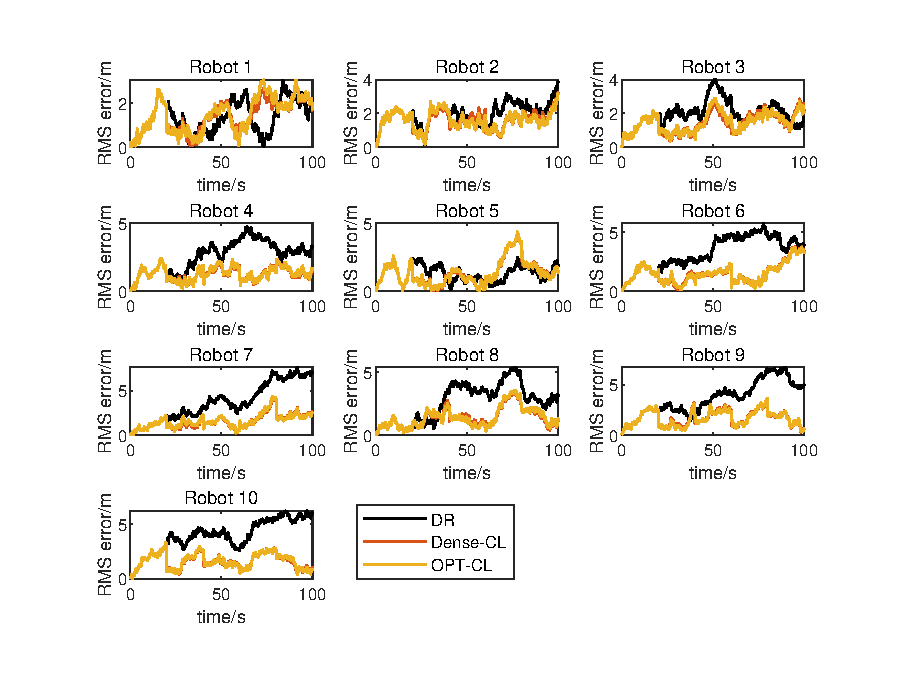
\includegraphics[width=3.7in]{Fig/fig2_rmse.eps}
	\caption{RMS Error}
	\label{fig::rmse}
\end{figure}
Figure \ref{fig::rmse} shows the DR,dense-CL and OPT-CL RMS error for all robots, in comparison to dead reckoning (abbreviated as 'DR' in hereafter plot legends).
As can be seen from the figure, after the measurement is initiated, the RMS error of most robots will drop significantly. The RMS caused by using dense-CL and OPT-CL is very close. For robots 4, 6, 7, 9, 10, the RMS is significantly lower after using the CL method. For robots 1, 2, and 5, the RMS does not decrease greatly, and it oscillates slightly at the RMS error level of DR. For robots 3 and 8, when using the CL method, the RMS error will increase relative to that of DR for a period of time after the measurement, but the overall RMS error is still lower than the original DR method.
\begin{figure}
	\centering
	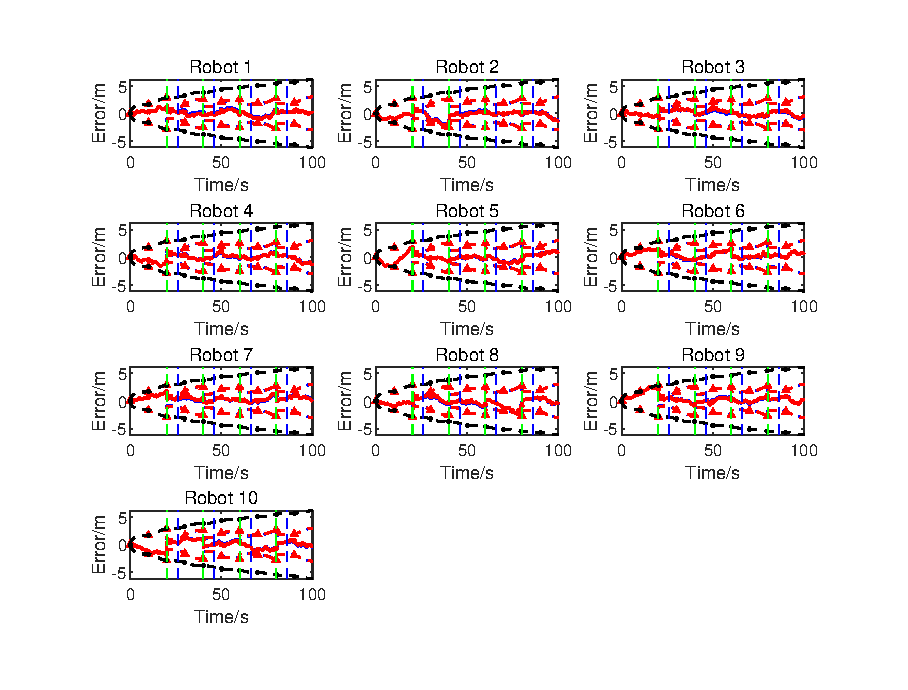
\includegraphics[width=3.7in]{Fig/fig3_3sigma.eps}
	\caption{Three sigma boundaries with estimation errors in X direction}
	\label{fig::3sigma}
\end{figure}

In Figure \ref{fig::3sigma}, three sigma boundaries as well as estimation errors in X direction are displayed.
The black, red and blue are the DR, dense-CL and OPT-CL 3-sigma bounds respectively. The red and blue solid line represents the estimation error of dense-CL and OPT-CL, which are all small enough to fit in the 3-sigma bound.
The green and blue dashed-lines stand for the start and end of CL respectively.
As one could see, the covariance of x coordinate estimation is bounded when CL is enabled and it would grow without bound when there is only propagation (DR).
The dense-CL has almost the same uncertainty growth as OPT-CL, with only minor difference when the under-threshold update happens.
\begin{figure}
	\centering
	\subfigure[Trace of covariance (zoomed out)]{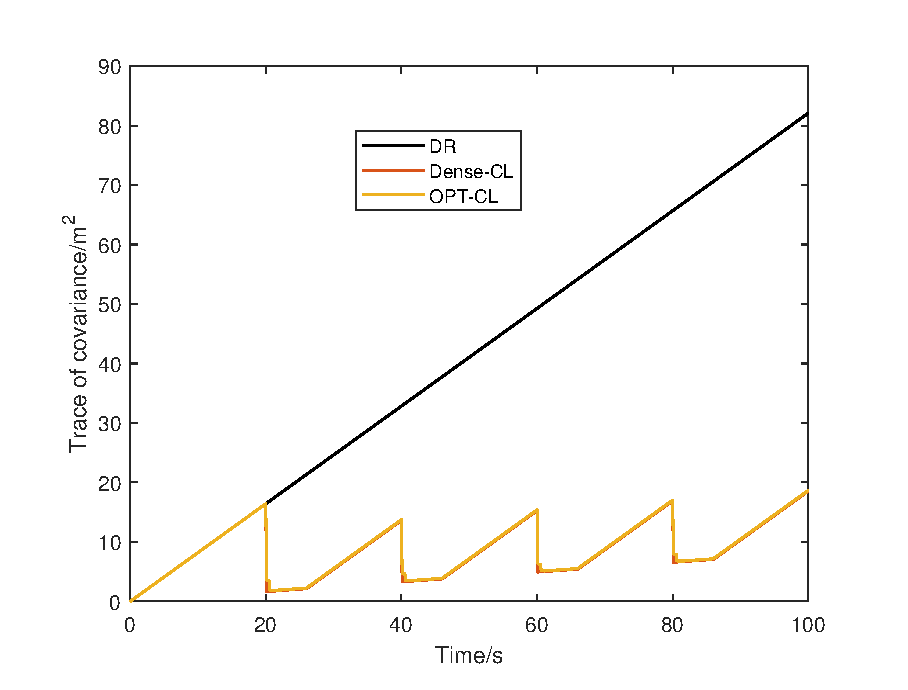
\includegraphics[width=3.7in]{Fig/fig4_trace.eps}}
	\subfigure[Trace of covariance (zoomed in)]{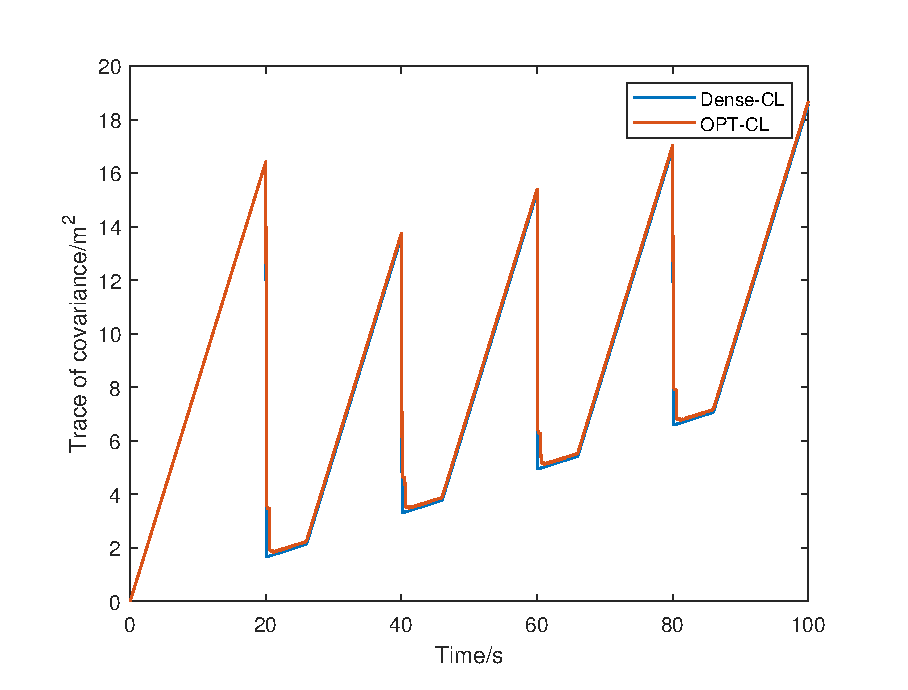
\includegraphics[width=3.7in]{Fig/fig4_trace_zoom_in.eps}}
	\caption{Trace of covariance and its upper bound}
	\label{fig::trace}
\end{figure}

Figure \ref{fig::trace} demonstrates the trace of covariance in multiple methods.
From the figure we can find that the trace of covariance of dense-CL behaves almost the same as OPT-CL's. But the trace of covariance of DR grows linearly as times go by.

\begin{figure}
	\centering
	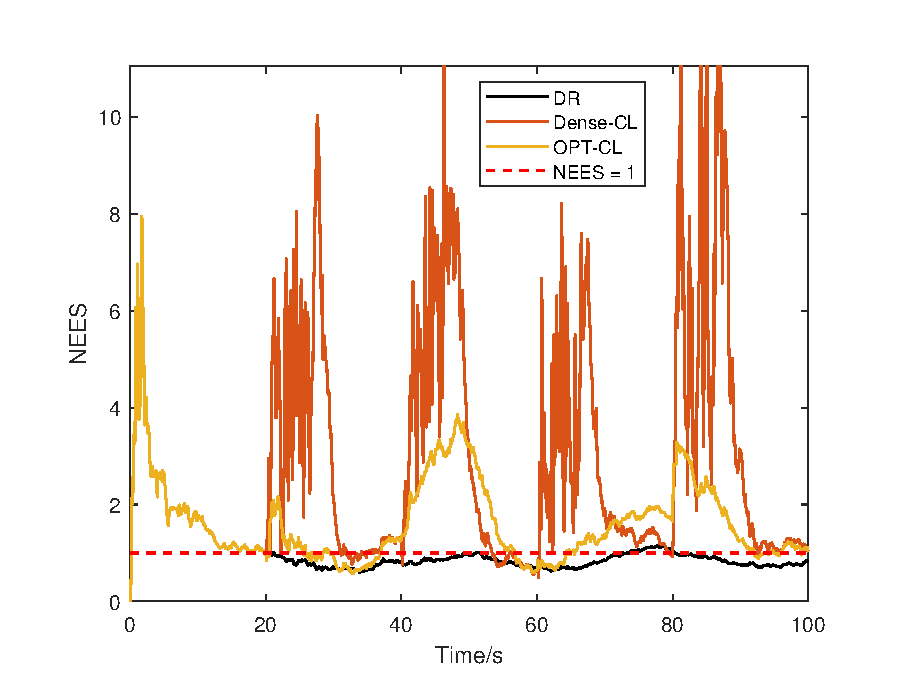
\includegraphics[width=3.7in]{Fig/fig5_nees.eps}
	\caption{NEES comparisons}
	\label{fig::nees}
\end{figure}

Figure \ref{fig::nees} represents the NEES (Normalized Estimation Error Squared) results of different methods. The NEES is a parameter that evaluates the performance of state estimation. The closer NEES is to 1, the better performance of state estimation.
As we can see from the figure, compared to dense-CL method, the NEES results of OPT-CL is much smaller and with less oscillation, which indicates that the OPT-CL performs better than dense-CL. 

\begin{figure}
	\centering
	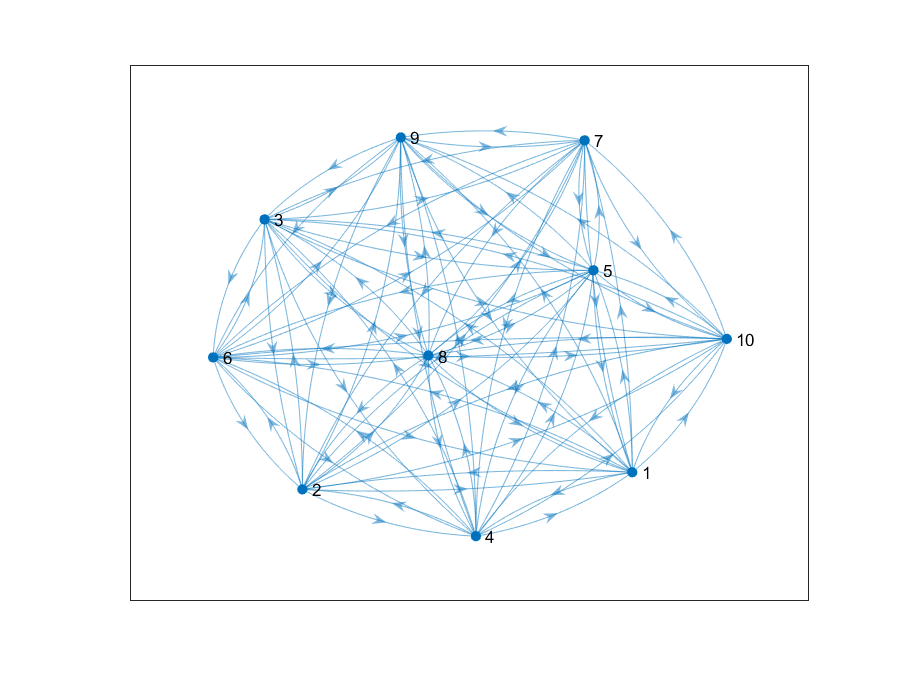
\includegraphics[width=3.5 in]{Fig/topology_dense.eps}
	\caption{Dense topology}
	\label{fig::dense_topology}
\end{figure}

\begin{figure}[H]
	\centering
	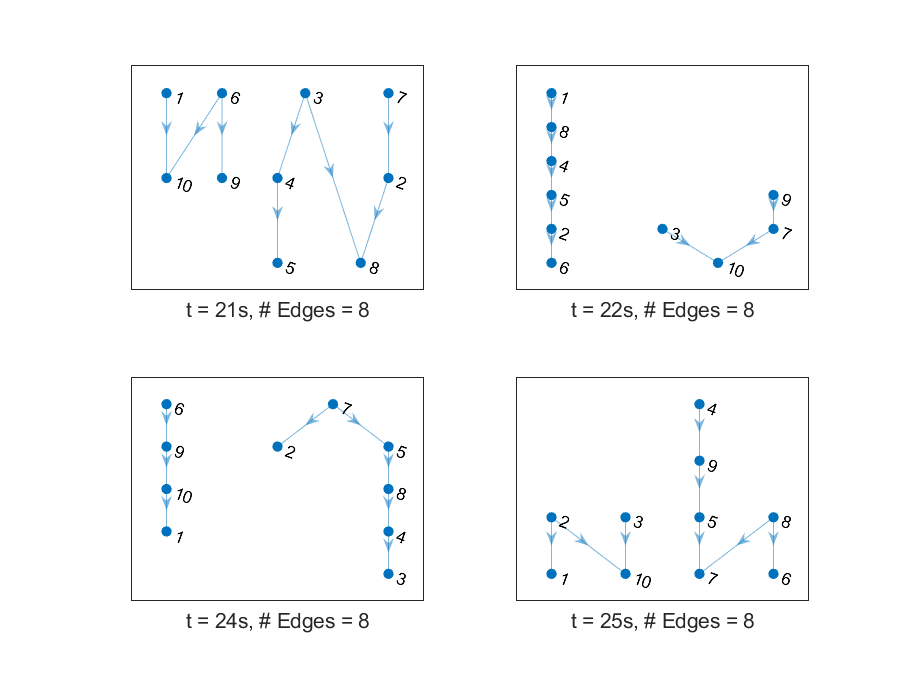
\includegraphics[width=3.5 in]{Fig/topology_sparse.eps}
	\caption{Sparse topology after optimization}
	\label{fig::sparse_topology}
\end{figure}
Figure \ref{fig::dense_topology} and Figure \ref{fig::sparse_topology} respectively represent the measurement network topology using DR and CL.
It can be seen that after optimization, the measurement network topology is much sparser than the original one, indicating that the number of measurements between the robots is significantly reduced. From the measurement network we can see that whether each robot initiates a measurement or whether it is being measured is uncertain. For example, the degrees of robot 2 is two outdegrees at t=24s, two indegrees at t=44s, and one indegree plus one outdegree at t=64s. Although the robot decides their measurements by the greedy selection approach, for any robot, the total degree is less than or equal to two. In this way, the number of mutual measurements is greatly reduced.

\section{Conclusions}
In this paper, we explicitly consider lowering the costs of CL algorithm from the novel prospective of dynamic topology switching method.
In our approach, the full-observability condition is not required unlike the past work, expanding the practicality of our method.
Moreover, a greedy approximation algorithm is constructed to gain a satisfiable solution to the optimization problem.
Numerical simulation validates the effectiveness of our proposed method.
In future, the work will consider detailed selection algorithm analysis such as worst-case performance analysis and full-state CL including relative orientation measurement.

\bibliographystyle{plainnat}
\bibliography{my_ref.bib}
\end{document}


